\section{Antecedentes de �rboles de decisi�n en S�ndrome Metab�lico}

Dentro de la planificaci�n y del an�lisis de los datos, se realizo una primera exploraci�n de los datos en donde, se decidi� evaluar la efectividad de un �rbol de decisi�n creado por el experto (esto es, un  endocrin�logo), y que fue validado por otro endocrinologo. La forma de realizaci�n de este �rbol fue  orientado puramente en caracter�sticas cl�nicas y no se tomaron en cuenta, las caracter�sticas bioqu�micas. \par
La raz�n de este desarrollo fue identificar: 1) que las variables cl�nicas no son suficientes para la adecuada clasificaci�n de los pacientes con s�ndrome metab�lico, y 2) a�n el experto necesita de una herramienta que mejore la capacidad predictiva en la vida diaria

\begin{figure}[h]
\centering
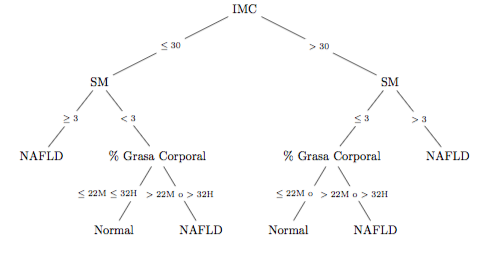
\includegraphics[height=5cm]{sm_dt}
\caption{�rbol de decisi�n creado por el experto}
\label{fig:sm_dt}
\end{figure}

En la figura \ref{fig:sm_dt} se logra ver que solo se cuentan con variables encontradas en la exploraci�n f�sica y que tambi�n pone en consideraci�n el g�nero de la persona. Todas las variables con caracter�sticas usadas por el Criterio de ATP III (Adult Treatment Panel III) para la clasificaci�n de s�ndrome metab�lico.\par

\begin{table}[h]
\centering
\begin{tabular}{|c|c|c|c|c|}\hline
Sensibilidad & Especificidad & VPP & VPN & Exactitud\\\hline
23\% & 78\% & 70\% & 31\% & 40.1\% \\\hline
\end{tabular}
\caption{Desempe�o del �rbol de decisi�n por el ATP III}
\label{tab:atp}
\end{table}

Como se observa en la tabla \ref{tab:atp}, este �rbol de decisi�n, no cuenta con suficiente exactitud para ser usado en todos los casos, aunque la especificidad del modelo es alta. El valor predictivo positivo tal vez nos permita considerarlo en ocasiones individuales.